\documentclass{beamer}
\usepackage[brazilian]{babel}
\usepackage[utf8]{inputenc}
\usepackage[T1]{fontenc}

\usetheme{Warsaw}

\title[Controlled Random Search]{Controlled Random Search na Inversão de Dados Magnetométricos}
\subtitle{Resolução do Exercício Proposto}
\author{Gean Lucas}
\institute{Observatório Nacional}
\date\today

\begin{document}
%\metroset{block=fill}

\begin{frame}
\titlepage
\end{frame}

\begin{frame}{Introduzindo o Controlled Random Search}
\begin{enumerate}
\item O Controlled Random Search é abreviado como CRS
\item Algoritmo desenvolvido por Price (1977) que usa modelos gerados aleatoriamente de forma controlada sendo mais eficiente do que algoritmos meramente aleatórios 
\item Projetado para priorizar uma busca mais profunda em detrimento da velocidade de convergência, por isso não é tão rápido quanto a maioria dos métodos \emph{derivativos}, mas tem uma chance mínima de parar num mínimo local
\end{enumerate}
\end{frame}

\begin{frame}{Aplicações do CRS}
O CRS tem aplicações em diversos problemas
\begin{enumerate}
\item Kim \emph{et al.} (2005) usaram o algoritmo CRS para determinar as configurações quase-ótimas dos parâmetros do processo de soldagem
\item O algoritmo também foi usado para otimizar modelos de regressão (Křivý e Tvrdík, 1995; Křivý \emph{et al}., 2000)
\item Em Merad et al. (2006), os autores formularam um problema de otimização para projetar arranjos de antenas lineares não uniformemente espaçados usando o algoritmo CRS
\end{enumerate}
\end{frame}

\begin{frame}{Aplicações do CRS}
Dentro as diversas aplicações, também temos a geofísica
\begin{enumerate}
\item Monteiro Santos and El-Kaliouby (2010) conclui que métodos aleatórios de busca global são os mais adequados para inversão conjunta 1D VES/TEM
\item Utilizado por Bortolozzo \emph{et al} (2015) para inversão conjunta 1D de dados de VES/TEM da Bacia do Paraná
\item Červ \emph{et al}. (2007) utilizaram o algoritmo CRS para inverter dados magnetotelúricos obtendo bons resultados
\item Smith e Ferguson (2000) demonstraram os benefícios do uso de CRS ao trabalhar com dados de sísmica de refração, especialmente quando focado na investigação de alvos específicos, o método CRS mostrou-se altamente eficaz na quantificação das estatísticas dos modelos
\end{enumerate}

\end{frame}


\begin{frame}{Aplicações do CRS}
\begin{enumerate}
\item Silva e Hohmann (1983) usaram CRS para interpretação magnética, concluindo que o algoritmo é muito robusto e, para o caso magnético, pode gerar ótimos resultados, especialmente quando informações geológicas e geofísicas estão disponíveis
\end{enumerate}
Todos os trabalhos que envolvem o algoritmo demonstram que os algoritmos de busca aleatória têm um desempenho muito bom e são robustos, pois dão grande determinação de parâmetro para problemas de otimização global mal estruturados (Bortolozzo \emph{et al.}, 2015)
\end{frame}

\begin{frame}{Motivação para escolha do CRS}
\begin{enumerate}
\item Conhecimento de prévio de aplicação em geofísica
\item ACO(Ant-Colony Optimization) se mostrou difícil de adaptar no curto prazo
\item Método randômico, comtemplando os métodos abordados na disciplina
\item Simples
\item Não requer cálculo de derivadas
\item Ampla gama de aplicação
\end{enumerate}
\end{frame}

\begin{frame}{Objetivo}
\begin{enumerate}
\item Implementar um programa computacional para a interpretação de um levantamento magnetométrico hipotético, usando um método randômico
\item O problema é determinar a “Coordenada horizontal” (xq), a “Profundidade” (zq) e o “Momento de Dipolo Magnético”(mom) de um corpo em sub superfície, a partir dos dados de um levantamento magnetométrico feito ao longo de um perfil Sul- Norte na direção do campo geomagnético, conforme a figura mostrada a seguir
\end{enumerate}
\end{frame}

\begin{frame}{Objetivo}
\begin{enumerate}
\item Ilustração do Problema
\end{enumerate}
\begin{center}
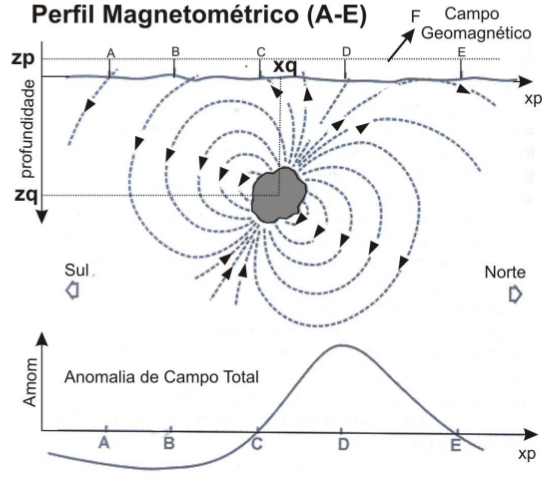
\includegraphics[scale=0.4]{problema}
\end{center}
\end{frame}

\begin{frame}{Método}
\begin{enumerate}
\item Utilizei o CRS
\item Tendo em mãos o modelo direto (subrotinas fornecidas pelo professor), pude equacionar a função objetivo 
\end{enumerate}

\begin{equation}
Anom = |B_{o}| - |F|
\end{equation}

Sendo:
\begin{enumerate}
\item $Anom =$ Anomalia de Campo Total
\item $B_{o} =$ Intensidade do Campo Observado
\item $F =$ Intensidade do Campo Geomagnético
\end{enumerate}

\end{frame}

\begin{frame}{Método}

\begin{equation}
norma = Rrms = \sqrt[2]{\frac{(Anom_{o} - Anom_{c})^2}{N}}  
\end{equation}

Sendo:
\begin{enumerate}
\item $Rrms =$ Residual root mean square
\item $Anom_{o} =$ Anomalia observada(obtida no levantamento)
\item $Anom_{c} =$ Anomalia calculada(calculada pelo modelo direto)
\item $N =$ Número de dados do levantamento
\end{enumerate}

\end{frame}

\begin{frame}{Método}
\begin{center}
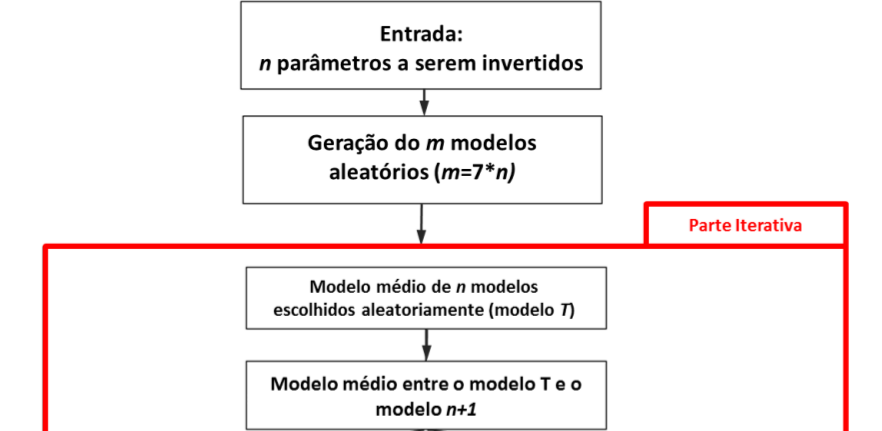
\includegraphics[scale=0.35]{esquema1}
\end{center}
\end{frame}

\begin{frame}{Método}
\begin{center}
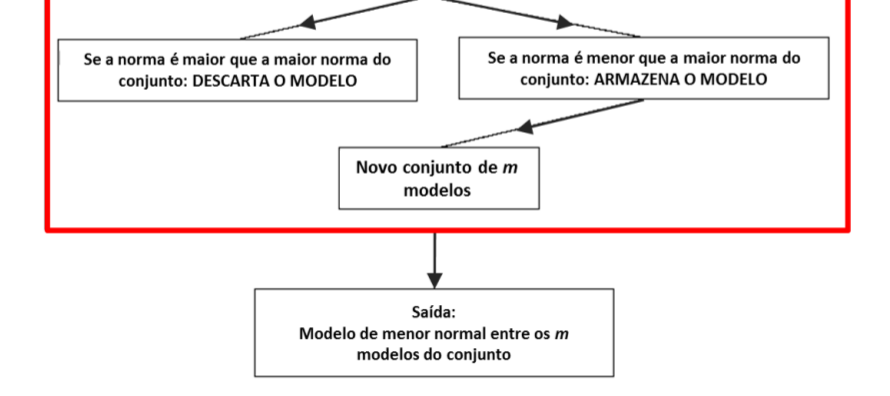
\includegraphics[scale=0.35]{esquema2}
\end{center}
\end{frame}

\begin{frame}{Método}
No entanto, no caso deste trabalho, na quarta etapa, o modelo final obtido antes da etapa da comparação foi:
\begin{center}
$P = 2*G - R_{n+1}$
Price (1976) and Collon (1992)
\end{center}
Onde:
\begin{enumerate}
\item $G$ corresponde ao $T$ do esquema anterior
\item $R_{n+1}$ corresponde a outro modelo escolhido aleatoriamente no conjunto de modelos (ou de pontos)
\end{enumerate}
\end{frame}

\begin{frame}{Resultados}
500 iterações
\begin{center}
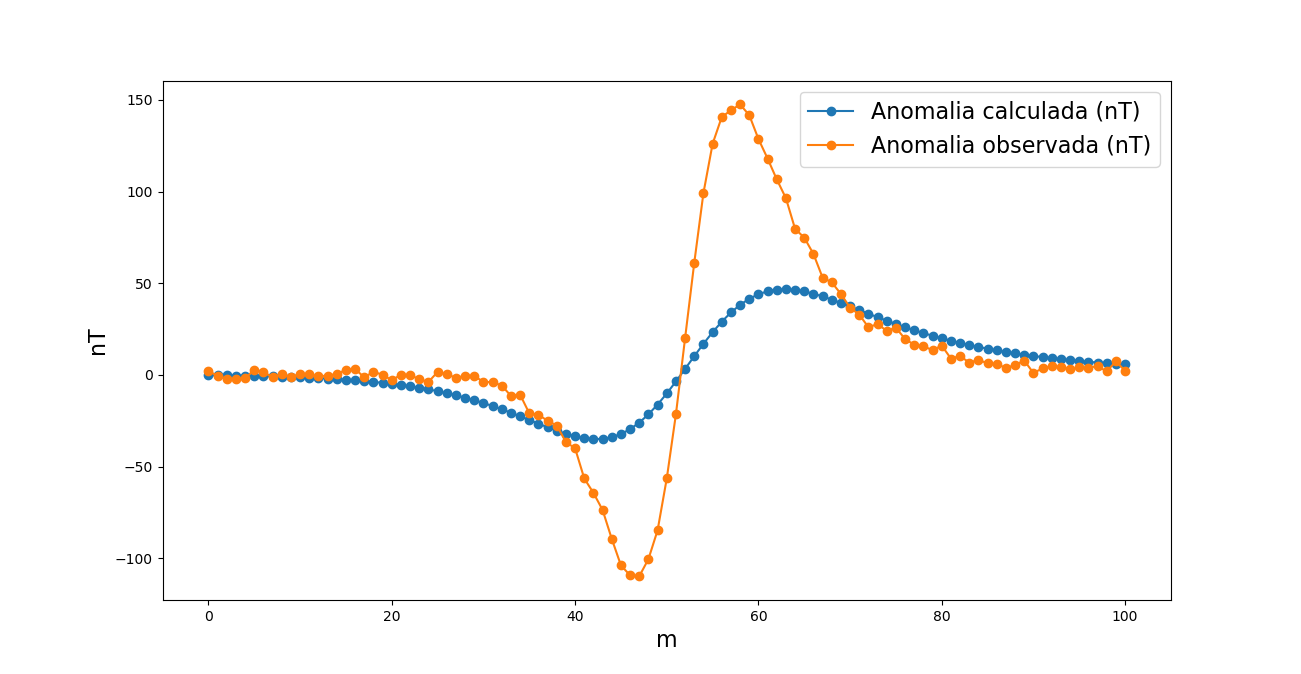
\includegraphics[scale=0.35]{500iteracoes}
\end{center}
\end{frame}

\begin{frame}{Resultados}
500 iterações
\begin{center}
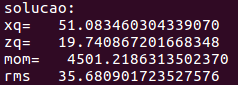
\includegraphics[scale=1]{rms_500}
\end{center}
\end{frame}

\begin{frame}{Resultados}
1000 iterações
\begin{center}
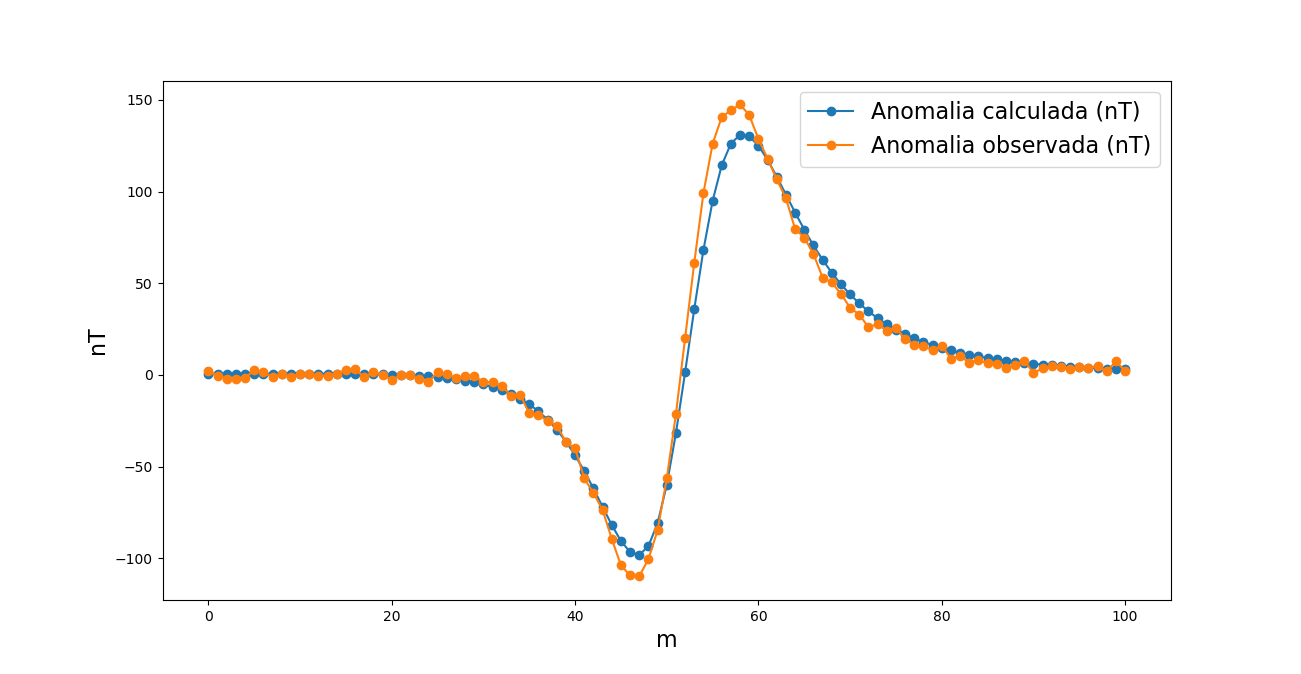
\includegraphics[scale=0.35]{1000iteracoes}
\end{center}
\end{frame}

\begin{frame}{Resultados}
1000 iterações
\begin{center}
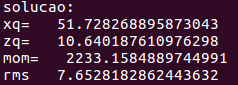
\includegraphics[scale=1]{rms_1000}
\end{center}
\end{frame}

\begin{frame}{Resultados}
5000 iterações
\begin{center}
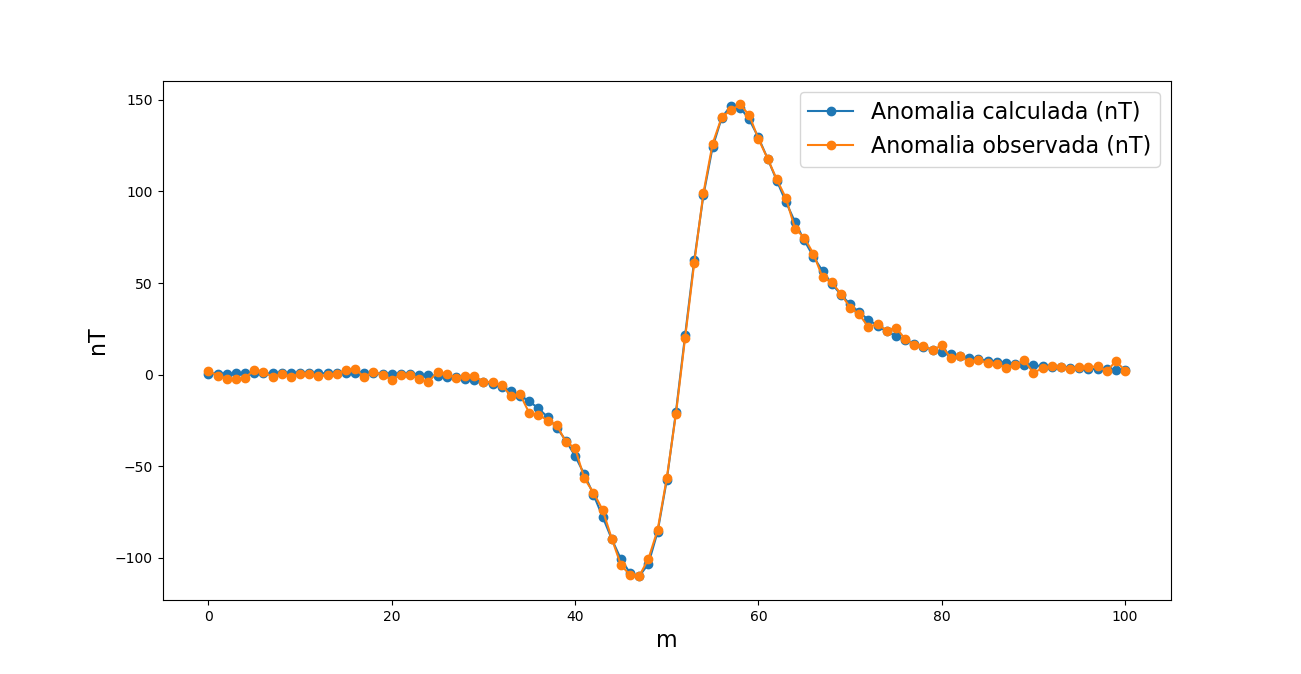
\includegraphics[scale=0.35]{5000iteracoes}
\end{center}
\end{frame}

\begin{frame}{Resultados}
5000 iterações
\begin{center}
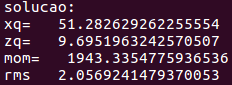
\includegraphics[scale=1]{rms_5000}
\end{center}
\end{frame}

\begin{frame}{Resultados}
10000 iterações
\begin{center}
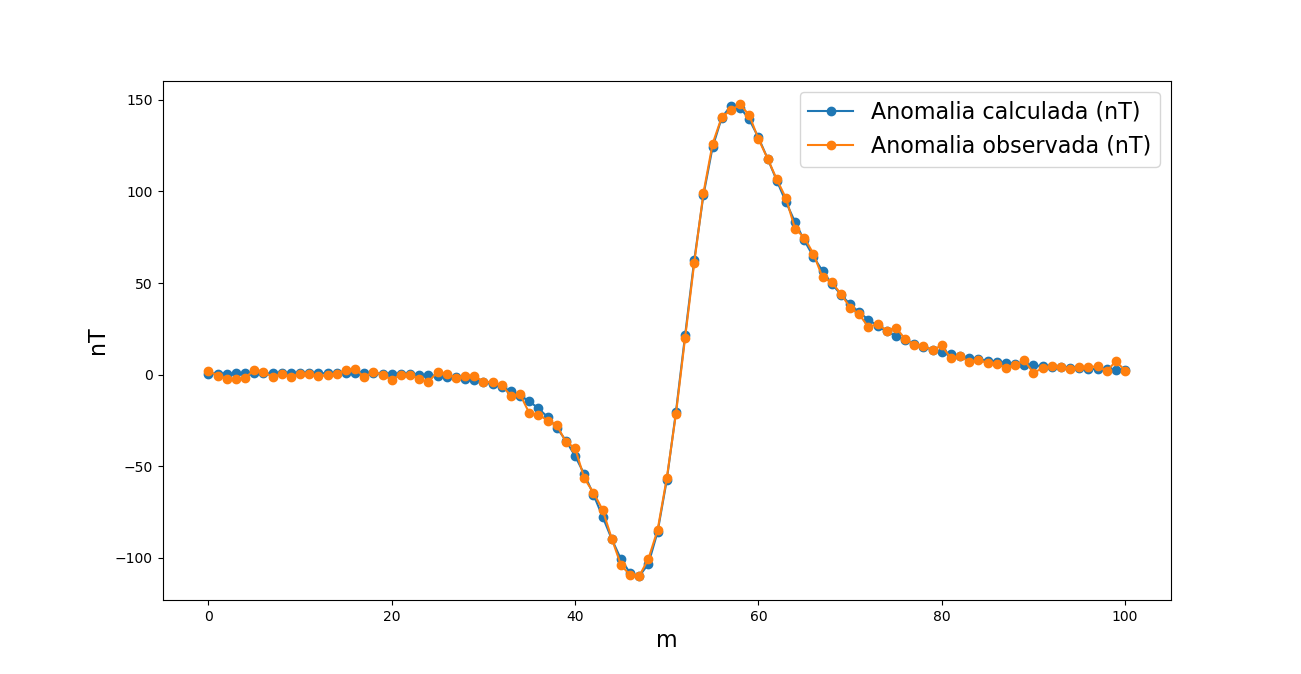
\includegraphics[scale=0.35]{10000iteracoes}
\end{center}
\end{frame}

\begin{frame}{Resultados}
10000 iterações
\begin{center}
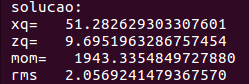
\includegraphics[scale=1]{rms_10000}
\end{center}
\end{frame}

\begin{frame}
Gráfico de convergência para 5000 iterações
\begin{center}
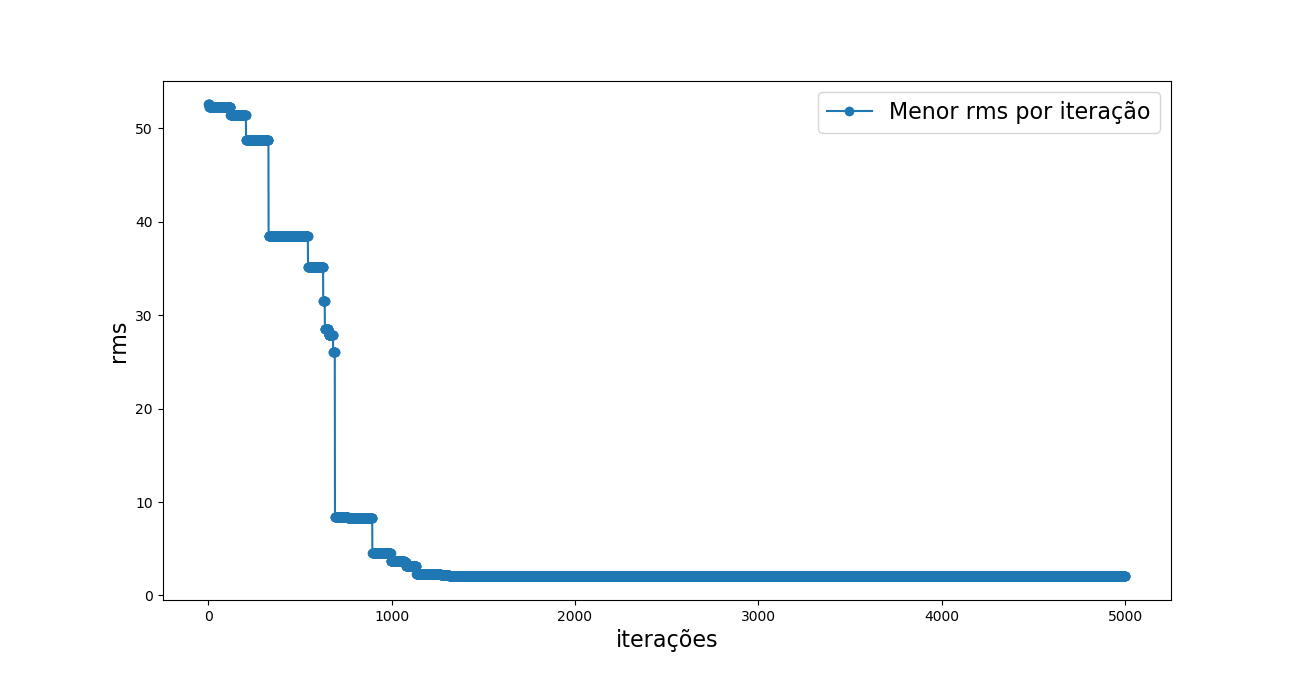
\includegraphics[scale=0.35]{conv}
\end{center}
\end{frame}

\begin{frame}{Referências}
\begin{enumerate}
\item Bortolozo, C. A., Porsani, J. L., dos Santos, F. A. M., & Almeida, E. R. (2015). VES/TEM 1D joint inversion by using Controlled Random Search (CRS) algorithm. Journal of Applied Geophysics, 112, 157-174.
\item Červ, V., Menvielle, M., Pek, J., 2007. Stochastic interpretation of magnetotelluric data, comparison of methods. Ann. Geophys. 50, 1.
\item Price, W.L., 1977. A controlled random search procedure for global optimization. Comput. J. 20, 367–370.
\item Smith, D.N., Ferguson, J.F., 2000. Constrained inversion of seismic refraction data using the controlled random search. Geophysics 65 (5), 1622–1630.
\item Silva, J.B.C., Hohmann, G.W., 1983. Nonlinear magnetic inversion using a random search method. Geophysics 48 (12), 1645–1658.
\end{enumerate}
\end{frame}

\end{document}